\chapter{Quantum Gases}

Quantum gases are systems of non-interacting or weakly interacting particles that obey quantum statistics. Depending on the nature of the particles, they can be classified as either bosons or fermions, leading to different statistical behaviors.

A quantum gas can be described using the grand canonical ensemble, where the number of particles can fluctuate, and the system is characterized by a fixed temperature \(T\), volume \(V\), and chemical potential \(\mu\); the Hamiltonian operator for a quantum gas of non-interacting particles can be expressed, for a fixed \(N\), as
\[
    \hat{H} = \sum_{i}^N \hat{\mathcal{O}}_i = \sum_{i}^N \left( \frac{\hat{p}_i^2}{2m} + U(\hat{q}_i) \right),
\]
where \(\hat{\mathcal{O}}_i\) is the single-particle operator, \(\hat{p}_i\) and \(\hat{q}_i\) are the momentum and position operators of the \(i\)-th particle, \(m\) is the mass of the particles, and \(U(\hat{q}_i)\) is the potential energy operator acting on the position of the \(i\)-th particle.

In second quantization, we can express the Hamiltonian operator in terms of creation and annihilation operators \(\hat{a}_{\alpha}^{\dagger}\) and \(\hat{a}_{\alpha}\) for the single-particle states:
\[
    \hat{H} = \sum_{\alpha \beta} t_{\alpha \beta} \hat{a}_{\alpha}^{\dagger} \hat{a}_{\beta},
\]
where the ladder operators satisfy the appropriate commutation or anticommutation relations depending on whether the particles are bosons or fermions: the nature of the particles determines the algebra of the creation and annihilation operators, which in turn affects the statistical properties of the quantum gas.
Looking at the ON base for the single-particle Hamiltonian \(\hat{\mathcal{O}}\), we can deduce a more useful form for our hamiltonian, diagonalized in terms of single-particle energy eigenstates \(\ket{e_{\alpha}}\) with eigenvalues \(\epsilon_{\alpha}\):
\[
    \hat{\mathcal{O}} \ket{e_{\alpha}} = \epsilon_{\alpha} \ket{e_{\alpha}},
\]
so that the full Hamiltonian operator can be expressed as
\[
    \hat{H} = \sum_{\alpha} \epsilon_{\alpha} \hat{a}_{\alpha}^{\dagger} \hat{a}_{\alpha},
\]
where \(\hat{a}_{\alpha}^{\dagger}\) and \(\hat{a}_{\alpha}\) are the creation and annihilation operators for the single-particle state \(\ket{e_{\alpha}}\), forming the number operator \(\hat{n}_{\alpha} = \hat{a}_{\alpha}^{\dagger} \hat{a}_{\alpha}\) that counts the number of particles in the state \(\ket{e_{\alpha}}\).

Thus we can define
\[
    \hat{H} - \mu \hat{N} = \sum_{\alpha} (\epsilon_{\alpha} - \mu) \hat{n}_{\alpha},
\]
where \(\hat{N} = \sum_{\alpha} \hat{n}_{\alpha}\) is the total number operator for the system.
The density operator for the quantum gas in the grand canonical ensemble is given by
\[
    \hat{\rho}_{gc} = \frac{1}{\mathcal{Z}} e^{-\beta (\hat{H} - \mu \hat{N})} = \frac{1}{\mathcal{Z}} e^{-\beta \sum_{\alpha} (\epsilon_{\alpha} - \mu) \hat{n}_{\alpha}},
\]
and the grandcanonical partition function can be computed as
\[
    \mathcal{Z} = \Tr_{\mathcal{F}}(e^{-\beta (\hat{H} - \mu \hat{N})}) = \Tr_{\mathcal{F}} \left( e^{-\beta \sum_{\alpha} (\epsilon_{\alpha} - \mu) \hat{n}_{\alpha}} \right),
\]
where we can construct the Fock space \(\mathcal{F}\) as the tensor product of the single-particle state spaces:
\[
    \ket{n_{1}, n_{2}, \ldots} = C (\hat{a}_{1}^{\dagger})^{n_1} (\hat{a}_{2}^{\dagger})^{n_2} \cdots \ket{0},
\],
with \(C\) a normalization constant and \(\ket{0}\) the vacuum state. The occupation numbers \(n_{\alpha}\) indicate how many particles occupy the single-particle state \(\ket{e_{\alpha}}\). Now we can compute the grand partition function exploiting the trace
\[
    \begin{aligned}
        \mathcal{Z} & = \sum_{n_1=0}^{n_{\text{max}}} \sum_{n_2=0}^{n_{\text{max}}} \cdots \bra{n_1, n_2, \ldots} e^{-\beta \sum_{\alpha} (\epsilon_{\alpha} - \mu) \hat{n}_{\alpha}} \ket{n_1, n_2, \ldots}                           \\
                    & = \sum_{n_1,\,n_2,\,\cdots} e^{-\beta \sum_{\alpha} (\epsilon_{\alpha} - \mu) n_{\alpha}} \bra{n_1, n_2, \ldots} \ket{n_1, n_2, \ldots}                                                                          \\
                    & = \sum_{n_1,\,n_2,\,\cdots} \prod_{\alpha} e^{-\beta (\epsilon_{\alpha} - \mu) n_{\alpha}} = \prod_{\alpha} \left( \sum_{n_{\alpha}=0}^{n_{\text{max}}} e^{-\beta (\epsilon_{\alpha} - \mu) n_{\alpha}} \right),
    \end{aligned}
\]
where we swapped the sums and products since the indices are independent (note how the sum changed index). The upper limit \(n_{\text{max}}\) of the sums over occupation numbers depends on the nature of the particles:
\begin{itemize}
    \item for bosons, \(n_{\text{max}} = \infty\), since multiple bosons can occupy the same quantum state;
    \item for fermions, \(n_{\text{max}} = 1\), due to the Pauli exclusion principle, which states that no two fermions can occupy the same quantum state simultaneously.
\end{itemize}

\section{Quantum Statistics}

We can now derive the specific forms of the grand partition function and related thermodynamic quantities for fermionic and bosonic quantum gases.
We need to compute the sum over occupation numbers for each case, rememnbering that we cannot accept divergences to infinity in the partition function, since it must be finite and well defined (imagine trying to compute the TD limit).

\paragraph{Fermionic case.}
For fermions, the occupation numbers \(n_{\alpha}\) can only take values 0 or 1. Therefore, the sum over occupation numbers for each single-particle state \(\alpha\) gives the following result grand partition function:
\[
    \mathcal{Z}_{F} = \prod_{\alpha} \left( \sum_{n_{\alpha}=0}^{1} e^{-\beta (\epsilon_{\alpha} - \mu) n_{\alpha}} \right) = \prod_{\alpha} \left( 1 + e^{-\beta (\epsilon_{\alpha} - \mu)} \right).
\]
From the grand partition function, we can derive the grand potential \(\Omega_F\) for the fermionic quantum gas, in order to relate thermodynamic quantities to the partition function:
\[
    \Omega_F = - \frac{1}{\beta} \log \mathcal{Z}_F = - \frac{1}{\beta} \sum_{\alpha} \log \left( 1 + e^{-\beta (\epsilon_{\alpha} - \mu)} \right).
\]
Now it is time to compute the average occupation number \(\langle n_{\alpha} \rangle\) for each single-particle state \(\alpha\) in the fermionic quantum gas. This quantity represents the expected number of particles occupying the state \(\ket{e_{\alpha}}\), and it's the core of \textbf{Fermi-Dirac statistics}:\footnote{The computation will be done after some result from the Bosonic case.}
\begin{equation}
    \langle n_{\alpha} \rangle_{F} = \frac{1}{e^{\beta (\epsilon_{\alpha} - \mu)} + 1}.
    \label{eq:fermi_dirac_distribution}
\end{equation}

\paragraph{Bosonic case.}
For bosons, the occupation numbers \(n_{\alpha}\) can take any non-negative integer value (0, 1, 2, ...). Therefore, the sum over occupation numbers for each single-particle state \(\alpha\) gives the following result for the grand partition function:
\[
    \mathcal{Z}_{B} = \prod_{\alpha} \left( \sum_{n_{\alpha}=0}^{\infty} e^{-\beta (\epsilon_{\alpha} - \mu) n_{\alpha}} \right) = \prod_{\alpha} \frac{1}{1 - e^{-\beta (\epsilon_{\alpha} - \mu)}},
\]
where we used the formula for the sum of a geometric series.\footnote{It is crucial that the series converges, it's not guaranteed for all values of \(\mu\) and \(\epsilon_{\alpha}\), and surely it's not only a way to reconduce to a prettier mathematical expression, as we will highlight.} Since the geometric series \(\sum_{n}x^n = \frac{1}{1-x}\) converges only for values of \(x < 1\), we get a prescription on the exponent:
\[
    e^{-\beta(\epsilon_{\alpha} - \mu)} < 1 \iff \epsilon_{\alpha} - \mu > 0 \iff \mu < \min_{\alpha}\{\epsilon_{\alpha}\},
\]
meaning that, since we can take \(\min_{\alpha}\{\epsilon_{\alpha}\} = 0\), the chemical potential \(\mu\) must be negative for the bosonic quantum gas to ensure convergence of the grand partition function; this condition has important physical implications, especially when considering phenomena like \textbf{Bose-Einstein condensation}.
From the grand partition function, we can derive the grand potential \(\Omega_B\) for the bosonic quantum gas:
\[
    \Omega_B = - \frac{1}{\beta} \log \mathcal{Z}_B = \frac{1}{\beta} \sum_{\alpha} \log \left( 1 - e^{-\beta (\epsilon_{\alpha} - \mu)} \right).
\]
Finally we get to derive the \textbf{Bose-Einstein statistics}, computing the average occupation number \(\langle n_{\alpha} \rangle\) for each single-particle state \(\alpha\) in the bosonic quantum gas:
\begin{equation}
    \langle n_{\alpha} \rangle_{B} = \frac{1}{e^{\beta (\epsilon_{\alpha} - \mu)} - 1}.
    \label{eq:bose_einstein_distribution}
\end{equation}

It is good practice to compact the expressions for the two different statistics in a single formula: from the grand partition function
\begin{equation}
    \mathcal{Z}_{B/F} = \prod_{\alpha} \left(1 \mp e^{-\beta(\epsilon_{\alpha} -\mu)}\right)^{\mp 1},
    \label{eq:quantum_gas_grandpartition}
\end{equation}
where the upper sign refers to bosons and the lower sign to fermions. Fo the grandpotential we have
\begin{equation}
    \Omega_{B/F} = \mp \frac{1}{\beta} \sum_{\alpha} \log \left(1 \pm e^{-\beta(\epsilon_{\alpha} - \mu)}\right),
    \label{eq:quantum_gas_grand_potential}
\end{equation}
and finally we are able to compute explucitly the average occupation number for both statistics at the same time:
\[
    \begin{aligned}
        \langle \hat{n}_{\alpha} \rangle^{B/F}_{gc} & = \Tr_{\mathcal{F}}(\rho_{gc} \hat{n}_{\alpha}) = \frac{1}{\mathcal{Z}_{B/F}} \Tr_{\mathcal{F}} \left( e^{-\beta (\hat{H} - \mu \hat{N})} \hat{n}_{\alpha} \right)                                      \\
                                                    & = \frac{1}{\mathcal{Z}_{B/F}} \Tr _{\mathcal{F}} \left( e^{-\beta \sum_{\gamma} (\epsilon_{\gamma} - \mu) \hat{n}_{\gamma}} \hat{n}_{\alpha} \right)                                                    \\
                                                    & = \frac{-1}{\beta\mathcal{Z}_{B/F}} \Tr_{\mathcal{F}}\left(\frac{\partial}{\partial \epsilon_{\alpha}} e^{-\beta \sum_{\gamma}(\epsilon_{\gamma} - \mu) \hat{n}_{\gamma}}\right)                        \\
                                                    & = \frac{-1}{\beta} \frac{\partial}{\partial \epsilon_{\alpha}} \log \mathcal{Z}_{B/F} = \frac{\partial}{\partial \epsilon_{\alpha}} \Omega_{B/F} = \frac{1}{e^{\beta (\epsilon_{\alpha} - \mu)} \mp 1},
    \end{aligned}
\]
where again the upper sign refers to bosons and the lower sign to fermions, recovering equations \eqref{eq:fermi_dirac_distribution} and \eqref{eq:bose_einstein_distribution}. We can now interpret these results: the average occupation number \(\langle n_{\alpha} \rangle\) gives the expected number of particles occupying the single-particle state \(\ket{e_{\alpha}}\) at thermal equilibrium. The difference in the denominators reflects the fundamental distinction between bosons and fermions:
\begin{itemize}
    \item For bosons, the minus sign in the denominator allows for the possibility of multiple particles occupying the same quantum state, leading to phenomena like Bose-Einstein condensation, where a macroscopic number of bosons can occupy the ground state at low temperatures.
    \item For fermions, the plus sign in the denominator enforces the Pauli exclusion principle, which prohibits multiple fermions from occupying the same quantum state. This leads to the characteristic filling of energy levels up to the Fermi energy at absolute zero temperature.
\end{itemize}

It is also interesting to analyze the behavior of these distributions compared to the classical Maxwell-Boltzmann distribution.
\begin{figure}[H]
    \centering
    \includegraphics[width=0.8\textwidth]{img/Quantum_and_classical_statistics.png}
    \caption{\small Comparison of quantum statistics (Fermi-Dirac and Bose-Einstein) with classical Maxwell-Boltzmann statistics. The plot illustrates how the average occupation number \(\langle n_{\alpha} \rangle\) varies with energy \(\epsilon_{\alpha}\) for different temperatures \(T\) and chemical potentials \(\mu\). At high energies or low densities, all three distributions converge, reflecting classical behavior. However, at low energies or high densities, quantum effects become significant, leading to deviations from classical predictions. Notably, the Bose-Einstein distribution allows for a divergence in occupation number as energy approaches the chemical potential, indicating the onset of Bose-Einstein condensation. In contrast, the Fermi-Dirac distribution approaches a maximum occupation of 1 due to the Pauli exclusion principle.}
    \label{fig:quantum_statistics_comparison}
\end{figure}

Let us compute the internal energy \(E\) of the quantum gas using the average occupation numbers derived above:
\[
    \begin{aligned}
        E & = \langle \hat{H} \rangle^{B/F}_{gc} = \Tr_{\mathcal{F}}(\rho_{gc} \hat{H}) = \frac{1}{\mathcal{Z}_{B/F}} \Tr_{\mathcal{F}} \left( e^{-\beta (\hat{H} - \mu \hat{N})} \hat{H} \right) \\
          & = - \frac{\partial}{\partial \beta} \log \mathcal{Z}_{B/F} \big\vert_z,
    \end{aligned}
\]
where the subscript \(\big\vert_z\) indicates that the derivative is taken at constant fugacity \(z = e^{\beta \mu}\). Expanding this expression, we have
\[
    \begin{aligned}
        E & = \frac{1}{\mathcal{Z}_{B/F}} \Tr_{\mathcal{F}} \left( e^{-\beta \sum_{\alpha} (\epsilon_{\alpha} - \mu) \hat{n}_{\alpha}} \sum_{\alpha} \epsilon_{\alpha} \hat{n}_{\alpha} \right) \\
          & = \sum_{\alpha} \epsilon_{\alpha} \left( \frac{1}{\mathcal{Z}_{B/F}} \Tr_{\mathcal{F}} \left( e^{-\beta (\hat{H} - \mu \hat{N})} \hat{n}_{\alpha} \right) \right)                   \\
          & = \sum_{\alpha} \epsilon_{\alpha} \langle \hat{n}_{\alpha} \rangle^{B/F}_{gc} = \sum_{\alpha} \frac{\epsilon_{\alpha}}{e^{\beta (\epsilon_{\alpha} - \mu)} \mp 1}.
    \end{aligned}
\]
So the internal energy of the quantum gas can be expressed as a sum over all single-particle states, weighted by their respective energies and average occupation numbers according to either Bose-Einstein or Fermi-Dirac statistics
\begin{equation}
    \langle \hat{H} \rangle^{B/F}_{gc} = \sum_{\alpha} \frac{\epsilon_{\alpha}}{e^{\beta (\epsilon_{\alpha} - \mu)} \mp 1},
    \label{eq:quantum_gas_internal_energy}
\end{equation}
where we have not made any assumptions about the specific form of the single-particle energy levels \(\epsilon_{\alpha}\); this expression is quite general and can be applied to various quantum gas systems, including those confined in different potentials or geometries. Let us now specialize to the case of non-relativistic 3D quantum gases confined in a cubic box of volume \(V = L^3\) with periodic boundary conditions.

\section{Non Relativistic 3D Quantum Gases}

For a non-relativistic quantum gas confined in a cubic box of volume \(V = L^3\) with periodic boundary conditions, the single-particle energy levels \(\epsilon_{\alpha}\) can be expressed in terms of the kinetic energy of the particles
\[
    \epsilon_{\mathbf{k}} = \frac{p^2}{2m} = \frac{\hbar^2 k^2}{2m},
\]
from the solution of the Schrödinger equation for a free particle in a box:
\[
    - \frac{\hbar^2 \nabla^2}{2m} \ket{\psi} = \epsilon \ket{\psi}.
\]
The allowed wavevectors \(\mathbf{k}\) are quantized due to the boundary conditions, leading to discrete energy levels given by
\[
    \mathbf{k} = \frac{2\pi}{L} (n_x, n_y, n_z), \quad n_x, n_y, n_z \in \mathbb{Z},
\]
so that the energy levels can be rewritten as
\[
    \epsilon_{\mathbf{k}} = \frac{\hbar^2}{2m} (k_x^2 + k_y^2 + k_z^2) \implies \epsilon_{\mathbf{n}} = \frac{\hbar^2}{2m} \left( \frac{2\pi}{L} \right)^2 (n_x^2 + n_y^2 + n_z^2).
\]

The key thermodynamic quantities for the quantum gas can be computed using the expressions derived earlier, substituting the specific form of the energy levels \(\epsilon_{\mathbf{n}}\): from the grand partition function
\[
    \mathcal{Z}_{B/F} = \prod_{\mathbf{n}} \left(1 \mp e^{-\beta(\epsilon_{\mathbf{n}} -\mu)}\right)^{\mp g},
\]
where \(g\) is the discrete degeneracy factor accounting for internal degrees of freedom (e.g., spin), we can derive the grand potential, internal energy, and average number of particles:
\[
    \begin{aligned}
        \Omega_{B/F} & = \pm \frac{g}{\beta} \sum_{\mathbf{n}} \log \left( 1 \mp e^{-\beta (\epsilon_{\mathbf{n}} - \mu)} \right), \\
        E_{B/F}      & = g\sum_{\mathbf{n}} \frac{\epsilon_{\mathbf{n}}}{e^{\beta (\epsilon_{\mathbf{n}} - \mu)} \mp 1},           \\
        N_{B/F}      & = g\sum_{\mathbf{n}} \frac{1}{e^{\beta (\epsilon_{\mathbf{n}} - \mu)} \mp 1}.
    \end{aligned}
\]

If we now consider the thermodynamic limit, where the volume \(V\) goes to infinity while keeping the particle density \(N/V\) constant, we can replace the sums over discrete states with integrals over continuous momentum space.
\[
    \sum_{\mathbf{k}} \to \sum_{\mathbf{n}} \xrightarrow{TD} (?)
\]
In order to perform this substitution, we need to determine the density of states in momentum space. The strategy is to look at the volume element in \(\mathbf{k}\)-space corresponding to each quantum state
\[
    \Delta k_j = \frac{2\pi}{L} \left((n_j + 1) - n_j \right) = \frac{2\pi}{L} \implies \Delta k_x \Delta k_y \Delta k_z = \left( \frac{2\pi}{L} \right)^3 = \frac{(2\pi)^3}{V},
\]
which in the thermodynamic limit becomes infinitesimal \(L \to \infty \implies \Delta k_j \to 0\). Therefore, the number of states in a volume element \(d^3k\) in \(\mathbf{k}\)-space is given by
\[
    \sum_{\mathbf{n}} \frac{\hbar^2}{2m} \left(\frac{2\pi}{L}\right)^3 (\Delta n_x)(\Delta n_y)(\Delta n_z) \longrightarrow \sum_{\mathbf{k}} \frac{V}{(2\pi)^3} (\Delta k_x) (\Delta k_y) (\Delta k_z),
\]
where we know that \((\Delta n_x)(\Delta n_y)(\Delta n_z) = 1\) since we are counting each discrete state and \((\Delta k_x)(\Delta k_y)(\Delta k_z)\) is the infinitesimal volume \(\mathrm{d}^3\mathbf{k}\) element in \(\mathbf{k}\)-space. Thus we pass from the sum over discrete states to an integral over continuous momentum space as
\[
    \sum_{\mathbf{k}} \longrightarrow \frac{V}{(2\pi)^3} \int \mathrm{d}^3 \mathbf{k}.
\]
We can use polar coordinates in momentum space, since the energy levels depend only on the magnitude of the wavevector \(k = |\mathbf{k}|\), leading to
\[
    \int \mathrm{d}^3 \mathbf{k} = 4\pi \int_0^{\infty} k^2 \mathrm{d}k \implies \sum_{\mathbf{k}} \longrightarrow \frac{V}{(2\pi)^3} 4\pi \int_0^{\infty} k^2 \mathrm{d}k = \frac{V}{2\pi^2} \int_0^{\infty} k^2 \mathrm{d}k.
\]
The final step is to change the integration variable from \(k\) to the energy \(\epsilon\), using the relation \(\epsilon = \frac{\hbar^2 k^2}{2m}\), which gives
\[
    k^2 \mathrm{d} k \to \left(\frac{2m}{\hbar^2}\right)^{3/2} \frac{\epsilon^{\tfrac12}}{2} \mathrm{d} \epsilon,
\]
so that we can express the sum over states as
\[
    \sum_{\mathbf{k}} \longrightarrow \frac{V}{2\pi^2} \left(\frac{2m}{\hbar^2}\right)^{3/2} \frac{1}{2} \int_0^{\infty} \epsilon^{\tfrac12} \mathrm{d} \epsilon = V \int g(\epsilon) \mathrm{d} \epsilon.
\]
Here, we have introduced the \textbf{density of states} \(g(\epsilon)\) for a non-relativistic 3D quantum gas, defined as
\begin{equation}
    g(\epsilon) = \frac{g}{4\pi^2} \left( \frac{2m}{\hbar^2} \right)^{3/2} \epsilon^{1/2} = A \epsilon^{1/2},
    \label{eq:3d_free_quantum_gas_density_of_states}
\end{equation}
which gives the number of available quantum states per unit energy interval at energy \(\epsilon\), where we have included the discrete degeneracy factor \(g\) from the internal degrees of freedom. For a generic system, the strategy to compute the density of states \(g(\epsilon)\) involves finding the relationship between the energy levels and the quantum numbers characterizing the states, then determining how many states fall within a given energy range (compute the volume in quantum number space corresponding to that energy range).

For a generic thermodynamic quantity that can be expressed as a sum over states \(\sum_{\alpha} f(\epsilon_{\alpha})\), we can now write it as an integral over energy using the density of states:
\[
    \sum_{\alpha} f(\epsilon_{\alpha}) \longrightarrow V \int_0^{\infty} g(\epsilon) f(\epsilon) \mathrm{d} \epsilon,
\]
so that we can express the grand potential, internal energy, and average number of particles for the non-relativistic 3D quantum gas in the thermodynamic limit as\footnote{Remember that the internal degeneracy factor \(g\) has already been included in the density of states \(g(\epsilon)\).}
\[
    \begin{aligned}
        \Omega_{B/F} & = \pm \frac{V}{\beta} \int_0^{\infty} g(\epsilon) \log \left( 1 \mp e^{-\beta (\epsilon - \mu)} \right) \mathrm{d} \epsilon, \\
        E_{B/F}      & = V \int_0^{\infty} g(\epsilon) \frac{\epsilon}{e^{\beta (\epsilon - \mu)} \mp 1} \mathrm{d} \epsilon,                       \\
        N_{B/F}      & = V \int_0^{\infty} g(\epsilon) \frac{1}{e^{\beta (\epsilon - \mu)} \mp 1} \mathrm{d} \epsilon.
    \end{aligned}
\]
These integrals can be evaluated using special functions, such as the polylogarithm function or power series, to obtain explicit expressions for the thermodynamic quantities of interest in terms of temperature, chemical potential, and volume.

Now, by some developments of these expressions, we can get interesting results and laws.

\paragraph{Equation of state.}
If we integrate by part the expression for the grandpotential \(\Omega_{B/F}\), we get
\[
    \begin{aligned}
        \Omega_{B/F} & = \pm \frac{AV}{\beta} \left[ \frac{2}{3} \epsilon^{\tfrac32} \log \left( 1 \mp e^{-\beta (\epsilon - \mu)} \right) \Big\vert_0^{\infty} \mp \int_0^{\infty} \frac{2}{3}\epsilon^{\tfrac32} \frac{\pm \beta e^{-\beta (\epsilon - \mu)}}{1 \mp e^{-\beta (\epsilon - \mu)}} \mathrm{d} \epsilon \right]                \\
                     & \qquad  \lim_{\epsilon \to \infty} \log(1 \mp 0) = 0 \quad \text{and} \quad \epsilon^{\tfrac32} \log(1 \mp e^{\beta \mu}) \Big\vert_{\epsilon = 0} = 0,                                                                                                                                                                \\
                     & \qquad A \tfrac{2}{3} \epsilon^{\tfrac32} = \tfrac{2}{3} \epsilon g(\epsilon),                                                                                                                                                                                                                                         \\
                     & = \mp \frac{V}{\beta} (\pm \beta) \frac{2}{3}\int_0^{\infty}g(\epsilon) \frac{\epsilon e^{-\beta (\epsilon - \mu)}}{1 \mp e^{-\beta (\epsilon - \mu)}} \mathrm{d} \epsilon = - \frac{2}{3} V \int_0^{\infty} g(\epsilon) \frac{\epsilon}{e^{\beta (\epsilon - \mu)} \mp 1} \mathrm{d} \epsilon = - \frac{2}{3}E_{B/F},
    \end{aligned}
\]
where we used the expression for the internal energy \(E_{B/F}\) in the last step. Thus we have derived an important relation between the grand potential and the internal energy for a non-relativistic 3D quantum gas: since the pressure \(p\) is related to the grand potential by \(p = - \frac{\Omega}{V}\), we can express the equation of state for the quantum gas as
\[
    pV = \frac{2}{3} E_{B/F}.
\]

\subsection{Power Series Expansion}

Now we have expressions for the thermodynamic quantities as integrals over energy, we can evaluate these integrals using power series expansions. We will analyze the average number of particles \(N_{B/F}/V = n_{B/F}\) and the pressure \(p_{B/F}\) in detail
\[
    \begin{aligned}
        n_{B/F} & = A \int_0^{\infty} \frac{\epsilon^{1/2}}{e^{\beta (\epsilon - \mu)} \mp 1} \mathrm{d} \epsilon,             \\
        p_{B/F} & = \frac{2}{3} A \int_0^{\infty} \frac{\epsilon^{3/2}}{e^{\beta (\epsilon - \mu)} \mp 1} \mathrm{d} \epsilon.
    \end{aligned}
\]
The idea is to perform a change of variable, since these expressions are impossible to evaluate directly written in this form (we will not get a simple solution, but a form from which it will be easy at least to compute the limits in temperature). Let us define the fugacity \(z = e^{\beta \mu}\) and perform the change
\[
    \beta \epsilon = x^2 \implies \beta \mathrm{d} \epsilon = 2x \mathrm{d}x,
\]
which will let us find a power series and also gaussian integrals, as we will show. Thus, it is possible to rewrite the expressions for the particle density and pressure as
\[
    \begin{aligned}
        n_{B/F} & = \mathcal{C} \int_0^{\infty} \frac{z x^2}{e^{x^2} \mp z} \mathrm{d} x = \mathcal{C} \int_0^{\infty} \frac{z x^2e^{-x^2}}{1 \mp ze^{-x^2}} \mathrm{d} x,                                 \\
        p_{B/F} & = \frac{2}{3\beta} \mathcal{C} \int_0^{\infty} \frac{zx^4}{e^{x^2} \mp z} \mathrm{d} x = \frac{2}{3\beta} \mathcal{C} \int_0^{\infty} \frac{zx^4e^{-x^2}}{1 \mp ze^{-x^2}} \mathrm{d} x,
    \end{aligned}
\]
where we have defined the constant\footnote{It comes from the change of variable, which left us with \(\frac{2A}{\beta^{3/2}} = 2 \frac{g}{4\pi^2} \left( \frac{2m}{\hbar^2} \right)^{3/2} \beta^{-3/2}\).}
\[
    \mathcal{C} = \frac{4g}{\sqrt{\pi}} \frac{1}{\lambda_{T}^3}, \quad \lambda_{T} = \sqrt{\frac{2\pi \hbar^2}{mk_B T}}.
\]
In both integrals we find the term \(\frac{z e^{-x^2}}{e^{-x^2}\mp z}\), which we can expand as a power series in \(z e^{-x^2}\) paying attention to the convergence conditions and the signs:
\begin{itemize}
    \item for bosons, we have
          \[
              \frac{z e^{-x^2}}{1 - z e^{-x^2}} = z e^{-x^2}\sum_{l=0}^{\infty} (z e^{-x^2})^l = \sum_{l=0}^{\infty} (z e^{-x^2})^{l+1},
          \]
          which converges for \(\vert z e^{-x^2} \vert < 1\), always true since \(z < 1\) for bosons;
    \item for fermions, we have
          \[
              \frac{z e^{-x^2}}{1 + z e^{-x^2}} = z e^{-x^2}\sum_{l=1}^{\infty} (-1)^{l} (z e^{-x^2})^l = \sum_{l=0}^{\infty} (-1)^{l} (z e^{-x^2})^{l+1},
          \]
          which converges for all \(z \notin ]-\infty,\, -1]\) for the alternating series, but since for fermions \(z > 0\) it always converges;
    \item we can thus write a single expression for both cases:
          \[
              \frac{z e^{-x^2}}{e^{-x^2} \mp z} = \sum_{l=0}^{\infty} (\pm 1)^{l} (z e^{-x^2})^{l+1}.
          \]
\end{itemize}
Substituting this series expansion into the integrals for \(n_{B/F}\) and \(p_{B/F}\), we get
\[
    \begin{aligned}
        n_{B/F} & = \mathcal{C} \sum_{l=0}^{\infty} (\pm 1)^{l} z^{l+1} \int_0^{\infty} x^2 e^{-(l+1)x^2} \mathrm{d} x,                  \\
        p_{B/F} & = \frac{2}{3\beta} \mathcal{C} \sum_{l=0}^{\infty} (\pm 1)^{l} z^{l+1} \int_0^{\infty} x^4 e^{-(l+1)x^2} \mathrm{d} x.
    \end{aligned}
\]
The integrals appearing in these expressions are standard gaussian integrals, which can be computed using the formula
\[
    \int_0^{\infty} x^{2n} e^{-ax^2} \mathrm{d} x = \frac{(2n-1)!!}{2^{n+1}} \sqrt{\frac{\pi}{a^{2n+1}}}, \quad a > 0,
\]
where \((x)!! = (x)(x - 2) \cdots 3 \cdot 1\) is the double factorial\footnote{Starting from \(2n-1\) we know it is an odd number and thus the product goes down by 2 each time until the unity.}. Applying this formula to our integrals, we find
\[
    \begin{aligned}
        \int_0^{\infty} x^2 e^{-(l+1)x^2} \mathrm{d} x & = \frac{\sqrt{\pi}}{4}\frac{1}{(l+1)^{3/2}},     \\
        \int_0^{\infty} x^4 e^{-(l+1)x^2} \mathrm{d} x & = \frac{3 \sqrt{\pi}}{8} \frac{1}{(l+1)^{5/2} }.
    \end{aligned}
\]
Substituting these results back into the expressions for \(n_{B/F}\) and \(p_{B/F}\), we obtain
\[
    \begin{aligned}
        n_{B/F} & = \mathcal{C} \sum_{l=1}^{\infty} (\pm 1)^{l} z^{l+1} \frac{\sqrt{\pi}}{4} \frac{1}{(l+1)^{3/2}} = \frac{g}{\lambda_{T}^3} \sum_{l=0}^{\infty} (\pm 1)^{l} \frac{z^{l+1}}{(l+1)^{3/2}},                         \\
        p_{B/F} & = \frac{2}{3\beta} \mathcal{C} \sum_{l=1}^{\infty} (\pm 1)^{l} z^{l+1} \frac{3\sqrt{\pi}}{8} \frac{1}{(l+1)^{5/2}} = \frac{g}{\beta \lambda_{T}^3} \sum_{l=0}^{\infty} (\pm 1)^{l} \frac{z^{l+1}}{(l+1)^{5/2}}.
    \end{aligned}
\]
These series expansions provide a way to compute the particle density and pressure of the quantum gas in terms of the fugacity \(z\) and temperature \(T\). They are particularly useful for analyzing the behavior of the system in different regimes, such as low or high temperatures, and for comparing the properties of bosonic and fermionic gases. We can make the notation lighter by defining the functions
\[
    \begin{aligned}
        f_{\nu}(z) & = \sum_{l=0}^{\infty} (-1)^{l} \frac{z^{l+1}}{(l+1)^{\nu}} \quad \text{(Fermions)}, \\
        g_{\nu}(z) & = \sum_{l=0}^{\infty} \frac{z^{l+1}}{(l+1)^{\nu}} \quad \text{(Bosons)},
    \end{aligned}
\]
so that we can rewrite the expressions for the particle density and pressure as
\[
    \begin{aligned}
        n_{B/F} & = \frac{g}{\lambda_{T}^3} \begin{dcases}
                                                f_{3/2}(z), & \text{(Fermions)}; \\
                                                g_{3/2}(z), & \text{(Bosons)};   \\
                                            \end{dcases}       \\
        p_{B/F} & = \frac{g}{\beta \lambda_{T}^3} \begin{dcases}
                                                      f_{5/2}(z), & \text{(Fermions)}; \\
                                                      g_{5/2}(z), & \text{(Bosons)}.   \\
                                                  \end{dcases}
    \end{aligned}
\]

\subsection{Classical Limit}

We can now analyze the classical limit of the quantum gas, by stopping at the first order (\(l=0\)) in the power series expansions derived above: this is justified because in the classical limit the fugacity \(z\) is much smaller than 1 (\(z \ll 1\)), so higher-order terms in the series become negligible. Thus, for the density we have
\[
    n = \frac{g}{\lambda_{T}^3} z \implies z = \frac{n \lambda_{T}^3}{g},
\]
which can be substituted back into the expressions for the pressure to obtain
\[
    p = \frac{g}{\beta \lambda_{T}^3} z = \frac{g}{\beta \lambda_{T}^3} \frac{n \lambda_{T}^3}{g} = \frac{n}{\beta} = n k_B T,
\]
recovering the classical ideal gas law \(pV = N k_B T\).

This limit corresponds to the regime where quantum effects are negligible, and the behavior of the gas can be described by classical statistics. The classical limit is typically valid when the thermal wavelength \(\lambda_{T} = \sqrt{\frac{2 \pi \hbar^2}{m k_B T}}\) is much smaller than the average interparticle distance, which occurs at \textbf{high temperatures or low densities}:
\[
    z \ll 1 \implies \text{ high } T \text{ or low } n.
\]
In this regime, both bosonic and fermionic quantum gases behave like classical ideal gases, and the differences in their quantum statistics become irrelevant: we can show this result explicitly by looking at the average occupation numbers for bosons and fermions in the limit \(z \ll 1\):
\[
    \langle n_{\alpha} \rangle^{B/F}_{gc} = \frac{1}{e^{\beta (\epsilon_{\alpha} - \mu)} \mp 1} \sim e^{-\beta (\epsilon_{\alpha}-\mu)} \quad \text{for } z \ll 1,
\]
which is the Maxwell-Boltzmann distribution for classical particles.

A final remark can be made about the expression of the chemical potential in the classical limit: since \(z = e^{\beta \mu} \ll 1\), we have \(\beta \mu \ll 0\) and thus we can recover
\[
    n = \frac{g}{\lambda_T^3} e^{\beta \mu} \implies \mu = - \frac{3}{2} k_B T \log \left( \frac{m k_B T}{2 \pi \hbar^2} \left(\frac{n}{g}\right)^{\tfrac{2}{3}} \right) \xrightarrow{T \to \infty} -\infty,
\]
which shows that in the classical limit the chemical potential diverges to negative infinity as the temperature increases.

\paragraph{Semiclassical expansion.}
If we now consider the next order in the power series expansions for the particle density and pressure, we can derive corrections\footnote{We are considering semiclassical limit, called like that beacause the statistic is almot classical, but we are in a regime where we cannot ignore contributions due to the quantum nature of the considered particles.} to the ideal gas law that account for quantum effects. Including the second term (\(l=1\)) in the series, we have
\[
    \begin{aligned}
        n_{B/F} & = \frac{g}{\lambda_{T}^3} \left( z \pm \frac{z^2}{2^{3/2}} \right),       \\
        p_{B/F} & = \frac{g}{\beta \lambda_{T}^3} \left( z \pm \frac{z^2}{2^{5/2}} \right).
    \end{aligned}
\]
Solving for \(z\) in terms of \(n\), we find
\[
    \frac{z^2}{2\sqrt{2}} \pm z \mp \frac{n \lambda_{T}^3}{g} = 0 \implies z = \sqrt{2} \left( \mp 1 \pm \sqrt{1 \pm \sqrt{2} \frac{n \lambda_{T}^3}{g}}\right),
\]
we solved the second order equation: the first and third signs are due to Bosonic or fermionic nature, the second to the choice of solution of the quadratic equation. Expanding the square root for small \(n \lambda_{T}^3/g\), since \(z \ll 1\) implies small \(n\), we can use the Taylor expansion of the radical \(\sqrt{1+x} \sim 1 + \frac{x}{2} - \frac{x^2}{8} + \cdots\) for \(x \ll 1\), leading to
\[
    z_{B/F} \sim \sqrt{2} \left[ \mp 1 \pm \left( 1 \pm \frac{1}{\sqrt{2}}\frac{n \lambda_{T}^3}{g} \mp \frac{1}{4} \left(\frac{n \lambda_{T}^3}{g}\right)^2 \right) \right] = \frac{n \lambda_{T}^3}{g} \mp \frac{1}{2\sqrt{2}} \left( \frac{n \lambda_{T}^3}{g} \right)^2.
\]
If we now substitute this expression for \(z\) back into the pressure, and keep terms up to second order in \(n \lambda_{T}^3/g\), we find
\[
    p_{B/F} = \frac{g}{\beta \lambda_{T}^3} \left[ \frac{n \lambda_{T}^3}{g} \mp \frac{1}{2\sqrt{2}} \left( \frac{n \lambda_{T}^3}{g} \right)^2 \pm \frac{1}{4\sqrt{2}} \left( \frac{n \lambda_{T}^3}{g} \right)^2 \right] = n k_B T \left[ 1 \mp \frac{n_{B/F}}{4\sqrt{2}}\frac{\lambda_{T}^3}{g} \right].
\]
This expression represents the semiclassical expansion of the equation of state for a quantum gas, showing how quantum statistics modify the ideal gas law. The correction term \(\mp \frac{n_{B/F}}{4\sqrt{2}}\frac{\lambda_{T}^3}{g}\) indicates that:
\begin{itemize}
    \item For bosons (upper sign), the pressure is reduced compared to the classical ideal gas, reflecting the tendency of bosons to cluster together in the same quantum state.
    \item For fermions (lower sign), the pressure is increased due to the Pauli exclusion principle, which prevents multiple fermions from occupying the same quantum state, leading to a higher effective pressure.
    \item These corrections become significant at low temperatures or high densities, where quantum effects dominate the behavior of the gas.
\end{itemize}
We get the idea of quantum gases being \textit{attractive} or \textit{repulsive} depending on their statistics, leading to different macroscopic behaviors compared to classical gases: it is not a real interaction between particles (we are studying free gases) but an effective behavior due to the underlying quantum statistics.

Thus the quantum corrections to the classical ideal gas law becomes small when:
\begin{enumerate}
    \item \(g\) is very large (high internal degeneracy): this reduces the effect of quantum statistics by providing more available states for the particles to occupy;\footnote{Fermions cannot occupy the same state, but if we have a very large degeneracy in the energy levels, then we can have a lot of fermions at the same energy, thus mimicking the Bosons behavior.}
    \item the thermal wavelength \(\lambda_{T}\) is very small (high temperature);\footnote{We are speaking of "small" and "large" in relative terms: we intend that \(\lambda_{T}\) is small compared to the Plank constant and other characteristic lengths of the system.}
    \item the particle density \(n\) is very small (low density, again leading to classical statistics).
\end{enumerate}

\section{Fermi-Dirac Gas}

When we are at very low temperatures, near absolute zero, the fugacity \(z = e^{\beta \mu}\) can approach or exceed unity, especially for bosons where \(\mu\) can be close to zero or positive. In this regime, the power series expansions for the thermodynamic quantities may not converge, leading to divergences in the computed values. We have to keep the whole power series
\[
    \begin{aligned}
        f_{\nu}(z) & = \sum_{l=0}^{\infty} (-1)^{l} \frac{z^{l+1}}{(l+1)^{\nu}} \quad \text{(Fermions)}, \\
        g_{\nu}(z) & = \sum_{l=0}^{\infty} \frac{z^{l+1}}{(l+1)^{\nu}} \quad \text{(Bosons)},
    \end{aligned}
\]
to obtain meaningful results.

\paragraph{Absolute convergence.}
We can study the absolute convergence of the series expansion (for both the Bose-Einstein functions $g_\nu(z)$ and the Fermi-Dirac functions $f_\nu(z)$) by considering the sum of the absolute values of its terms. Since the alternating sign $(\pm 1)^l$ vanishes inside the modulus, we obtain:
\[
    \sum_{l=0}^{\infty} \left\vert (\pm 1)^{l}\frac{z^{l+1}}{(l+1)^{\nu}} \right\vert = \sum_{l=0}^{\infty} \frac{\vert z \vert^{l+1}}{(l+1)^{\nu}}.
\]
Applying the standard ratio test,\footnote{The standard ratio test consists in taking the limit of the absolute value of the fraction \(a_{n+1}/a_n\), and then checking if this limit is less than 1 for convergence.} this series converges absolutely if and only if:
\[
    \lim_{l \to \infty} \left| \frac{z^{l+2}}{z^{l+1}} \left(\frac{l+1}{l+2}\right)^{\nu} \right| \sim \vert z \vert < 1.
\]
While for Bosons this series is always convergent (they always satisfy $\vert z \vert < 1$, since $\mu \le 0$), for Fermions the fugacity \(z\) can take any positive value, including values greater than 1 when the chemical potential \(\mu\) is positive. Therefore, we have absolute convergence only for \(\vert z \vert < 1\). For \(z > 1\), the series may or may not be \textit{simply convergent}, and it can be necessary to evaluate the functions \(f_{\nu}(z)\) using the integral representation (analytic continuation) rather than this power series.

Thus, for fermions in the classical regime the series converges absolutely for all physically relevant values of \(z\).
\begin{figure}[H]
    \begin{minipage}[c]{0.5\textwidth}
        \centering
        \includegraphics[width=0.8\textwidth]{img/fermions_power_series.jpg}
    \end{minipage}
    \hfill
    \begin{minipage}[c]{0.45\textwidth}
        \caption{Plot of the Fermi-Dirac power series \(f_{\nu}(z)\) for different values of \(\nu\) in the classical limit. If the series is well defined and convergent for all \(z \geq 0\), then it is positive, continuous and monotonically increasing. For \(z\) near 0 the series assumes a linear behavior, while for large \(z\) it grows more slowly.}
        \label{fig:figure-fermi-dirac-series}
    \end{minipage}
\end{figure}

We are looking at the limit for small temperatures \(T \to 0\), such that \(\beta \to \infty\) and thus \(z = e^{\beta \mu} \to \infty\) if \(\mu > 0\):\footnote{Remember for the following computation that the discrete internal degeneracy is included in \(A\) or \(g(\epsilon)\).} recalling the integral expressions for the particle density and energy density (since they are valid for all temperatures in general)
\[
    \begin{aligned}
        n  = \frac{N}{V}       & = A \int_0^{\mu} \d{\epsilon} \epsilon^{1/2} \frac{1}{e^{\beta(\epsilon-\mu)} + 1} = \int_0^{\infty} \d{\epsilon}g(\epsilon)\langle n(\epsilon) \rangle^{FD}_{gc},           \\
        \epsilon = \frac{E}{V} & = A \int_0^{\mu} \d{\epsilon} \epsilon^{3/2} \frac{1}{e^{\beta(\epsilon-\mu)} + 1} = \int_0^{\infty} \d{\epsilon}g(\epsilon) \langle n(\epsilon) \rangle^{FD}_{gc} \epsilon,
    \end{aligned}
\]
where it is crucial to know that the \textit{density of states} \(g(\epsilon)\) has unique definitions valid for the system under consideration (remember we are in the non-relativistic 3D quantum gas setting).
Now it is of maximum interest to understand how \(\langle n(\epsilon) \rangle^{FD}_{gc}\) behaves in this limit: plotting the function for \(\beta \to \infty\), and we find that it behaves as a \textit{Heaviside step function}
\[
    \langle n(\epsilon) \rangle^{FD}_{gc} = \frac{1}{e^{\beta(\epsilon - \mu)} + 1} = \begin{dcases}
        1,   & \epsilon < \mu; \\
        1/2, & \epsilon = \mu; \\
        0,   & \epsilon > \mu.
    \end{dcases}
\]
This is the famous \textbf{Fermi-Dirac distribution at zero temperature}, which shows that all states with energy below the chemical potential \(\mu\) are fully occupied, while those above \(\mu\) are empty. The chemical potential at zero temperature is known as the \textbf{Fermi energy} \(\epsilon_F\), which defines the highest occupied energy level in the system at absolute zero.

\begin{figure}[H]
    \begin{minipage}[c]{0.5\textwidth}
        \centering
        \includegraphics[width=0.8\textwidth]{img/FD_distribution_0K.png}
    \end{minipage}
    \hfill
    \begin{minipage}[c]{0.45\textwidth}
        \caption{Plot of the Fermi-Dirac distribution at zero temperature, which resembles a Heaviside step function. All states with energy below the chemical potential \(\mu\) (the Fermi energy \(\epsilon_F\)) are fully occupied, while those above are empty; while we let \(T\) increase the step function smooths out as thermal excitations allow some particles to occupy higher energy states.}
        \label{fig:figure-fermi-dirac-zero-temp}
    \end{minipage}
\end{figure}

Thus, we can compute the integrals for \(n\) and \(\epsilon\) at zero temperature as
\[
    \begin{aligned}
        n        & = \int_0^{\mu=\epsilon_F} g(\epsilon) \cdot 1 \, \mathrm{d} \epsilon = A \int_0^{\mu} \epsilon^{1/2} \mathrm{d} \epsilon = \frac{2}{3} A \epsilon_F^{3/2},          \\
        \epsilon & = \int_0^{\mu=\epsilon_F} g(\epsilon) \epsilon \cdot 1 \, \mathrm{d} \epsilon = A \int_0^{\mu} \epsilon^{3/2} \mathrm{d} \epsilon = \frac{2}{5} A \epsilon_F^{5/2}.
    \end{aligned}
\]
We can also find an explicit expression for the Fermi energy \(\epsilon_F\) in terms of the particle density \(n\):
\[
    \epsilon_F = \left( \frac{3n}{2A} \right)^{2/3},
\]
so that we can control the behavior of the system at zero temperature acting on the density of particles.
\begin{figure}[H]
    \begin{minipage}[c]{0.60\textwidth}
        \centering
        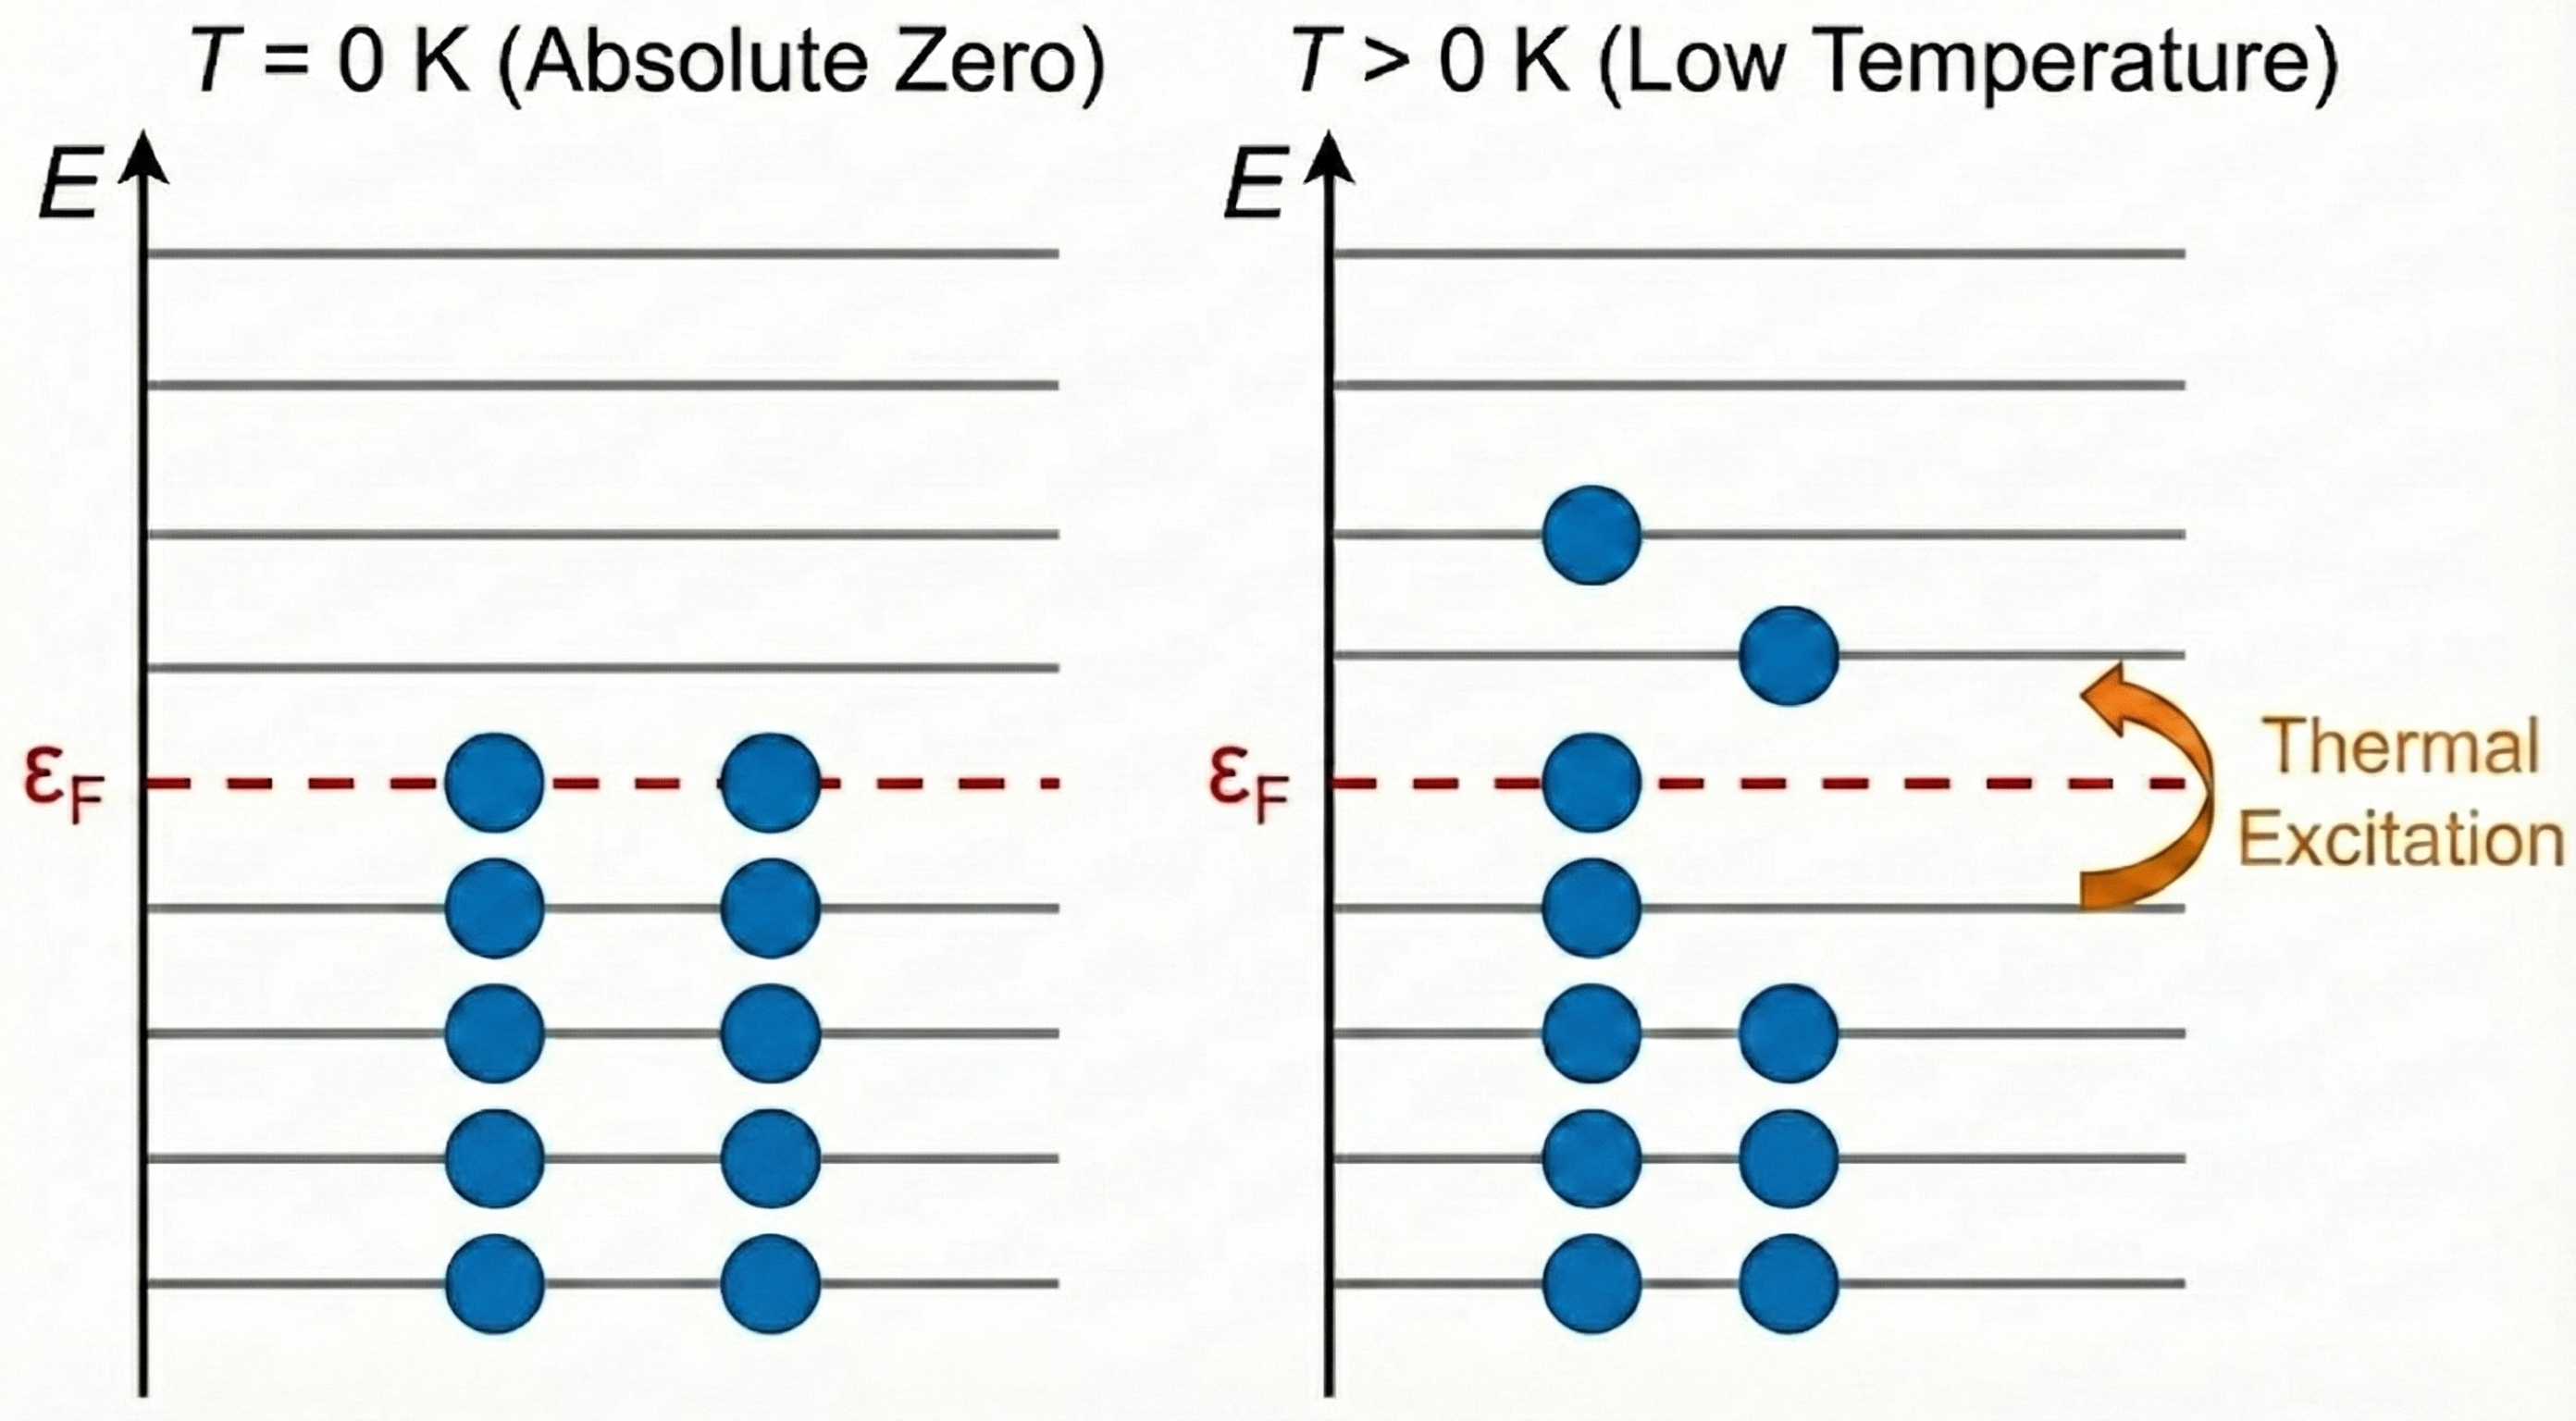
\includegraphics[width=0.8\textwidth]{img/fermi_occupation_levels.png}
    \end{minipage}
    \hfill
    \begin{minipage}[c]{0.35\textwidth}
        \caption{Occupation of energy levels by electrons in a metal at zero temperature, illustrating the filling up to the Fermi energy \(\epsilon_F\). As temperature increases, electrons can be thermally excited to higher energy states above \(\epsilon_F\).}
    \end{minipage}
\end{figure}
We can study how metals behave under these conditions, since the conduction electrons in metals can be modeled as a Fermi gas. At low temperatures, the electrons fill up energy levels up to the Fermi energy, leading to unique electronic properties, such as electrical conductivity and heat capacity, which differ significantly from classical predictions. We can dope the metal to change the electron density \(n\), which in turn modifies the Fermi energy \(\epsilon_F\) and thus the electronic properties of the material.
\begin{figure}[H]
    \begin{minipage}[c]{0.25\textwidth}
        \caption{Band diagram of a semiconductor showing the Fermi level in relation to the conduction band and valence band.}
    \end{minipage}
    \hfill
    \begin{minipage}[c]{0.70\textwidth}
        \centering
        \includegraphics[width=0.8\textwidth]{img/Semiconductor_Fermi_Level_Band_Diagram.jpg}
    \end{minipage}
\end{figure}

We can also compute the grand potential \(\Omega_F\) at zero temperature using the relation \(\Omega_F = - \frac{2}{3} E_F\) with the intent to find the pressure of the Fermi gas at absolute zero:
\[
    \Omega_F = - \frac{2}{3} V \epsilon = - pV, \quad p = \frac{2}{3}\epsilon = \frac{2}{3} \left(\frac{3}{5}n \epsilon_F\right) = \frac{2}{5} n \epsilon_F > 0.
\]
For any perfect classical gas we have a zero pressure at zero temperature, while here we have a finite pressure due to the Pauli exclusion principle, which prevents all fermions from occupying the lowest energy state. This leads to a degeneracy pressure that supports the system against collapse, which is particularly important in astrophysical contexts such as white dwarf stars: the electron degeneracy pressure arising from the Fermi gas of electrons counteracts gravitational collapse, stabilizing the star.

\paragraph{Fermi temperature.}
With an augment in temperature, the sharp occupation of energy levels at the Fermi energy smooths out, leading to thermal excitations around \(k_B T\) of electrons near the Fermi level, affecting the electronic properties of the material. It is thus really useful to define a Fermi temperature \(T_F\) associated to the Fermi energy:
\[
    k_B T_F = \epsilon_F \implies T_F = \frac{\epsilon_F}{k_B},
\]
which provides a temperature scale below which quantum effects become significant for the fermi gas. At temperatures much lower than \(T_F\), the gas exhibits quantum behavior, with non negligible behaviours due to statistical properties, while at temperatures much higher than \(T_F\), it behaves more classically
\[
    T_F = \frac{1}{k_B}\left(\frac{6\pi^2}{g}\right)\frac{\hbar^2}{2m}n^{2/3}.
\]
This fact is not arbitrary: it comes from the comparison between the thermal energy \(k_B T\) and the Fermi energy \(\epsilon_F\), in the denominator of the Fermi-Dirac distribution. When \(k_B T \ll \epsilon_F\), the thermal excitations are small compared to the energy scale set by the Fermi energy, leading to quantum behavior. Conversely, when \(k_B T \gg \epsilon_F\), thermal excitations dominate, and the gas behaves more classically (i.e. the occupation of energy levels follows the Maxwell-Boltzmann distribution):
\[
    \frac{1}{e^{\beta(\epsilon - \mu)} + 1} \xrightarrow{k_B T \gg \epsilon_F} e^{-\beta(\epsilon - \mu)},
\]
considering \(\epsilon\) near the Fermi energy.

We can derive an approximate value for a metal with \(n \sim 10^{22 / 23} \text{ electron}/\text{cm}^3\), \(g=2\) (for spin degeneracy) and \(m\) equal to the electron mass:
\[
    T_F \sim 10^{4-5} K,
\]
so that at room temperature (\(\sim 300 K\)) the electron gas in metals can be treated as a degenerate Fermi gas, with quantum effects dominating its behavior.
For stars like white dwarfs, where the electron density is extremely high (\(n \sim 10^{30} \text{ electron}/\text{cm}^3\)), the Fermi temperature can reach values on the order of \(10^{11} K\) or higher (where the star temperature is much lower, around \(10^7\) Kelvin), indicating that the electron gas remains degenerate even at very high temperatures.

\section{Bose-Einstein Gas}

We can now analyze the behavior of a Bose gas at low temperatures, where quantum effects become significant and lead to phenomena such as Bose-Einstein condensation. Starting from the expressions for the particle density and the pressure:
\[
    \begin{aligned}
        n & = \frac{g}{\lambda_{T}^3} g_{3/2}(z),       \\
        p & = \frac{g}{\beta \lambda_{T}^3} g_{5/2}(z),
    \end{aligned}
\]
where again we have defined the Bose-Einstein functions \(g_{\nu}(z)\) as a power series in the fugacity \(z\):
\[
    g_{\nu}(z) = \sum_{l=0}^{\infty} \frac{z^{l+1}}{(l+1)^{\nu}}.
\]
We can study the behavior of these functions as \(z\) approaches 1 (low temperatures) and as \(z\) is very small compared to 1 (high temperatures). These are the two regimes of interest for the Bose gas: the quantum degenerate regime and the classical limit. We will start with the classical limit, which we have already analyzed in general terms, and then we will focus on the quantum degenerate regime where characteristic effects of bosons emerge.

\subsection{Classical and Semiclassical Limits}

In the classical limit, where \(z = e^{\beta \mu} \ll 1\) since the temperature is high, we can approximate the Bose-Einstein functions by considering only the first term in the power series:
\[
    g_{\nu}(z) \approx z \quad \text{for } z \ll 1.
\]
Substituting this approximation into the expressions for the particle density and pressure, we recover the classical ideal gas law:
\[
    \begin{aligned}
        n & \approx \frac{g}{\lambda_{T}^3} z,       \\
        p & \approx \frac{g}{\beta \lambda_{T}^3} z.
    \end{aligned}
\]
Solving for \(z\) in terms of \(n\), we find
\[
    z \approx \frac{n \lambda_{T}^3}{g},
\]
which can be substituted back into the expression for the pressure to obtain
\[
    p \approx n k_B T,
\]
recovering the classical ideal gas law \(pV = N k_B T\).

We can also find an expression for the chemical potential in the classical limit:
\[
    z = e^{\beta \mu} \approx \frac{n \lambda_{T}^3}{g} \implies \mu \approx k_B T \log \left( \frac{n \lambda_{T}^3}{g} \right) = - \frac{3}{2} k_B T \log \left( \frac{m k_B T}{2 \pi \hbar^2} \left(\frac{g}{n}\right)^{\tfrac{2}{3}} \right) \xrightarrow{T \to \infty} -\infty.
\]
This shows that in the classical limit the chemical potential diverges to negative infinity as the temperature increases.
Finally, if we consider the Bose-Einstein distribution for the average occupation number of a single-particle state:
\[
    \langle n_{\alpha} \rangle^{B}_{gc} = \frac{1}{e^{\beta (\epsilon_{\alpha} - \mu)} - 1} \sim e^{-\beta (\epsilon_{\alpha}-\mu)} \quad \text{for } z \ll 1,
\]
we recover the Maxwell-Boltzmann distribution for classical particles.

If we now consider the next order in the power series expansion for the Bose-Einstein functions, we can derive semiclassical corrections to the ideal gas law that account for quantum effects. Practically, we are working in the regime in which particles are behaving almost classically but small quantum corrections are needed to be taken into account: we are approaching the quantum degenerate regime. Including the second term (\(l=1\)) in the series, we have
\[
    \begin{aligned}
        n & \approx \frac{g}{\lambda_{T}^3} \left( z + \frac{z^2}{2^{3/2}} \right),       \\
        p & \approx \frac{g}{\beta \lambda_{T}^3} \left( z + \frac{z^2}{2^{5/2}} \right).
    \end{aligned}
\]
Solving for \(z\) in terms of \(n\), and substituting this expression for \(z\) back into the pressure (keeping terms up to second order in \(n \lambda_{T}^3/g\)) we find the same expression derived previously for the general quantum gas, but now specified for bosons:
\[
    p = n k_B T \left[ 1 + \frac{n}{4\sqrt{2}}\frac{\lambda_{T}^3}{g} \right].
\]
This expression represents the semiclassical expansion of the equation of state for a Bose gas, showing how quantum statistics modify the ideal gas law. The correction term \(+ \frac{n}{4\sqrt{2}}\frac{\lambda_{T}^3}{g}\) indicates that for bosons, the pressure is increased compared to the classical ideal gas, reflecting the tendency of bosons to cluster together in the same quantum state. These corrections become significant at low temperatures or high densities, where quantum effects dominate the behavior of the gas.

\subsection{Quantum Regime}

To analyze the behavior of the Bose gas in the quantum degenerate regime, we need to consider the full power series expansion for the Bose-Einstein functions \(g_{\nu}(z)\): we need to check convergence of the series as \(z\) approaches 1 (low temperatures). The series converges for all \(z < 1\), but as \(z\) approaches 1, the terms in the series become larger and larger, leading to a divergence at \(z = 1\).

We will consider both the particle density and pressure expressions, so we need the series expansion for both \(g_{3/2}(z)\) and \(g_{5/2}(z)\). Starting from the general expression
\[
    g_{\nu}(z) = \sum_{l=0}^{\infty} \frac{z^{l+1}}{(l+1)^{\nu}},
\]
we have to analyze \(\nu=3/2\) and \(\nu=5/2\):
\begin{enumerate}
    \item For \(\nu = 3/2\):
          \[
              g_{3/2}(z) = \sum_{l=0}^{\infty} \frac{z^{l+1}}{(l+1)^{3/2}}.
          \]
          As \(z\) approaches 1, the series diverges, indicating that the particle density \(n\) also diverges. In particular
          \begin{itemize}
              \item For \(\vert z \vert < 1\), the series is \textbf{absolutely convergent};
              \item For \(\vert z \vert = 1\), the series is \textbf{simply convergent};
              \item For \(\vert z \vert > 1\), the series is \textbf{divergent}.
          \end{itemize}
          These properties should not surprise us, since bosons can have \(\mu(T) \leq 0\) and thus \(z \leq 1\): the only physically relevant case is the first one, where the series converges absolutely.
    \item For \(\nu = 5/2\):
          \[
              g_{5/2}(z) = \sum_{l=0}^{\infty} \frac{z^{l+1}}{(l+1)^{5/2}}.
          \]
          Similar considerations apply here: as \(z\) approaches 1, the series diverges, indicating that the pressure \(p\) also diverges. The series diverges as \(\vert z \vert\) grows, but it is defined for all values of the fugacity, even for \(\vert z \vert > 1\).
\end{enumerate}

We now intend to study the dependence of the \textbf{chemical potential} \(\mu\) on the temperature \(T\) in this quantum degenerate regime.
\begin{itemize}
    \item At high temperatures, we are in the classical limit where \(\mu \to -\infty\) as \(T \to \infty\), leading to \(z \ll 1\).
    \item As the temperature decreases, \(\mu\) increases towards 0, leading to an increase in the fugacity \(z\) towards 1.
    \item The chemical potential is a monotonically decreasing function of temperature
          \[
              \frac{\partial \mu}{\partial T} \leq 0,
          \]
          approaching 0 from below as \(T\) approaches a critical temperature \(T_c\).
\end{itemize}
\TODO{insert plot of mu vs T for Bose gas.}
Thus we can define the critical temperature \(T_c\) for Bose-Einstein condensation as the temperature at which the chemical potential \(\mu\) reaches 0, leading to \(z = 1\); there are two possible cases:
\begin{itemize}
    \item \(T_c = 0\) so that \(\mu(T_c)=0\) \(\implies\) we are in the \(2D\)-Bose gas case, where no condensation occurs at finite temperature (we will show this later);
    \item \(T_c \neq 0\) so that \(\mu(T_c)=0\) \(\implies\) we are in the \(3D\)-Bose gas case, where condensation occurs at a finite temperature (below \(T_c\)).
\end{itemize}
Setting our analysis in the \(3D\) case, we can find an expression for the critical temperature \(T_c\) by setting \(\mu = 0\) (thus \(z=1\)) in the expression for the particle density:
\[
    n = \frac{g}{\lambda_{T_c}^3} g_{3/2}(1) = \frac{g}{\lambda_{T_c}^3} \zeta(3/2),
\]
where we have used the Riemann zeta function \(\zeta(\nu) = \sum_{l=0}^{\infty} \frac{1}{(l+1)^{\nu}}=g_{\nu}(1)\) to express \(g_{3/2}(1)\). Solving for \(T_c\), we find
\[
    T_{BEC} = \frac{2 \pi \hbar^2}{m k_B} \left( \frac{n}{g \zeta(3/2)} \right)^{2/3}.
\]
This expression shows that the critical temperature for \textbf{Bose-Einstein condensation} depends on the particle density \(n\), the mass of the bosons \(m\), and the internal degeneracy \(g\). Below this temperature, a macroscopic number of bosons occupy the ground state, leading to the phenomenon of Bose-Einstein condensation, which has been observed experimentally in systems such as ultracold atomic gases. This happens at temperatures comprised in the range of nanoKelvins to microKelvins, since the chemical potential remains equal to zero in this whole range of temperatures below \(T_{BEC}\).

So the occupation number for temperatures below \(T_{BEC}\) can be expressed as
\[
    n(T<T_{BEC}) = \frac{g}{\lambda_{T}^3} \zeta(3/2).
\]
We have to pay attention reading the consequences of this result: as temperature decreases below \(T_{BEC}\) and approaches absolute zero, \(\lambda_T = \left(\frac{2\pi\hbar^2}{m k_B T}\right)^{1/2}\xrightarrow{T \to 0} \infty\) diverges, leading to a decrease in the particle density \(n\) until the absolute zero is reached:
\[
    n \xrightarrow{\lambda_T \to \infty} 0.
\]
Particles cannot disappear as temperature decreases, so we have to conclude that the expression for the particle density above only accounts for particles in excited states (with \(\epsilon > 0\)), while a macroscopic number of particles condense into the ground state (with \(\epsilon = 0\)). If we consider, indeed, the number of particles in the ground state for \(\epsilon = 0\), we can write
\[
    \langle n_0 \rangle_{gc}^{B} = \frac{1}{e^{\beta(0 - \mu)} - 1} = \frac{1}{e^{-\beta \mu} - 1} = \frac{z}{1 - z} \xrightarrow{z \to 1} \infty,
\]
indicating that as \(\mu\) approaches 0 (i.e., as \(z\) approaches 1), the occupation number of the ground state diverges, leading to a macroscopic occupation of this state. But we can be more precise: the total number of particles \(N\) in the system can be expressed as the sum of particles in the ground state \(N_0\) and particles in excited states \(N_{exc}\): starting again from the number of states in the momentum space
\[
    N = \sum_{\mathbf{k}} n(\epsilon_{\mathbf{k}}), \quad \epsilon_{\mathbf{k}} = \frac{\hbar^2 \mathbf{k}}{2m}, \quad \mathbf{k} = \frac{2\pi}{L} (n_x,\, n_y,\, n_z),
\]
if we compute the TD limit the number of particles becomes
\[
    N = \int_0^{\infty} \d{\epsilon} g(\epsilon) \langle n(\epsilon) \rangle_{gc}^{B} = N_0 + \int_{\epsilon > 0} \d{\epsilon} g(\epsilon) \langle n(\epsilon) \rangle_{gc}^{B} = N_0 + N_{exc}.
\]
This is the crucial point: since \(\langle n(0) \rangle_{gc}^{B}\Big\vert_{\mu=0} \to \infty\) we formally need to separate the contribution of the ground state (with \(\epsilon = 0\)) from the contributions of all excited states (with \(\epsilon > 0\)), even if the integral over all energies wasn't seeing the divergence: it is only one point and computing the integral does not capture the divergence. Thus, we can express the number of particles as
\[
    N = N_0 + \sum_{\mathbf{k}} \epsilon_{\mathbf{k}},
\]
\(N_0\) being the number of particles in the ground state, and the sum being over all excited states. In the TD limit, the number of particles divided by the volume becomes
\[
    n = n_0(T) + \frac{1}{V} \int_0^{\infty} \d{\epsilon} g(\epsilon) \langle n(\epsilon) \rangle_{gc}^{B},
\]
and if we now take the limit \(\mu \to 0\) (thus \(z \to 1\)) we find
\[
    n = n_0(T) + \frac{g}{\lambda_{T}^3} \zeta(3/2) = n_0(T) + n_{n}(T),
\]
since we call the number of particles in excited states \(n_{n}(T)\), the "\textbf{normal}" component of the gas.
If we compute the normal density for temperatures below \(T_{BEC}\), the number of particles in excited states is given by
\[
    n_{n}(T < T_{BEC}) = \frac{g}{\lambda_{T}^3} \zeta(3/2) = \frac{g}{\lambda_{T_{BEC}}^3} \frac{n \lambda_T^3}{g} = n \left( \frac{T}{T_{BEC}} \right)^{3/2},
\]
indicating that not all particles can be accommodated in excited states, leading to a macroscopic occupation of the ground state:
\[
    n_0 = n - n_{n} = n \left[ 1 - \left( \frac{T}{T_{BEC}} \right)^{3/2} \right].
\]
This expression shows that as the temperature decreases below \(T_{BEC}\), the number of particles in the ground state \(N_0\) increases, reaching a maximum of \(N\) at absolute zero. This phenomenon is the hallmark of Bose-Einstein condensation, where a significant fraction of bosons occupy the lowest energy state, leading to unique macroscopic quantum phenomena such as superfluidity and coherence.

------